\begin{enumerate}
	\item{
	%Part a
		Convert circuit to its s domain equivalent, and assume no energy stored at $t=0^-$:
		\begin{figure}[H]
			\centering
			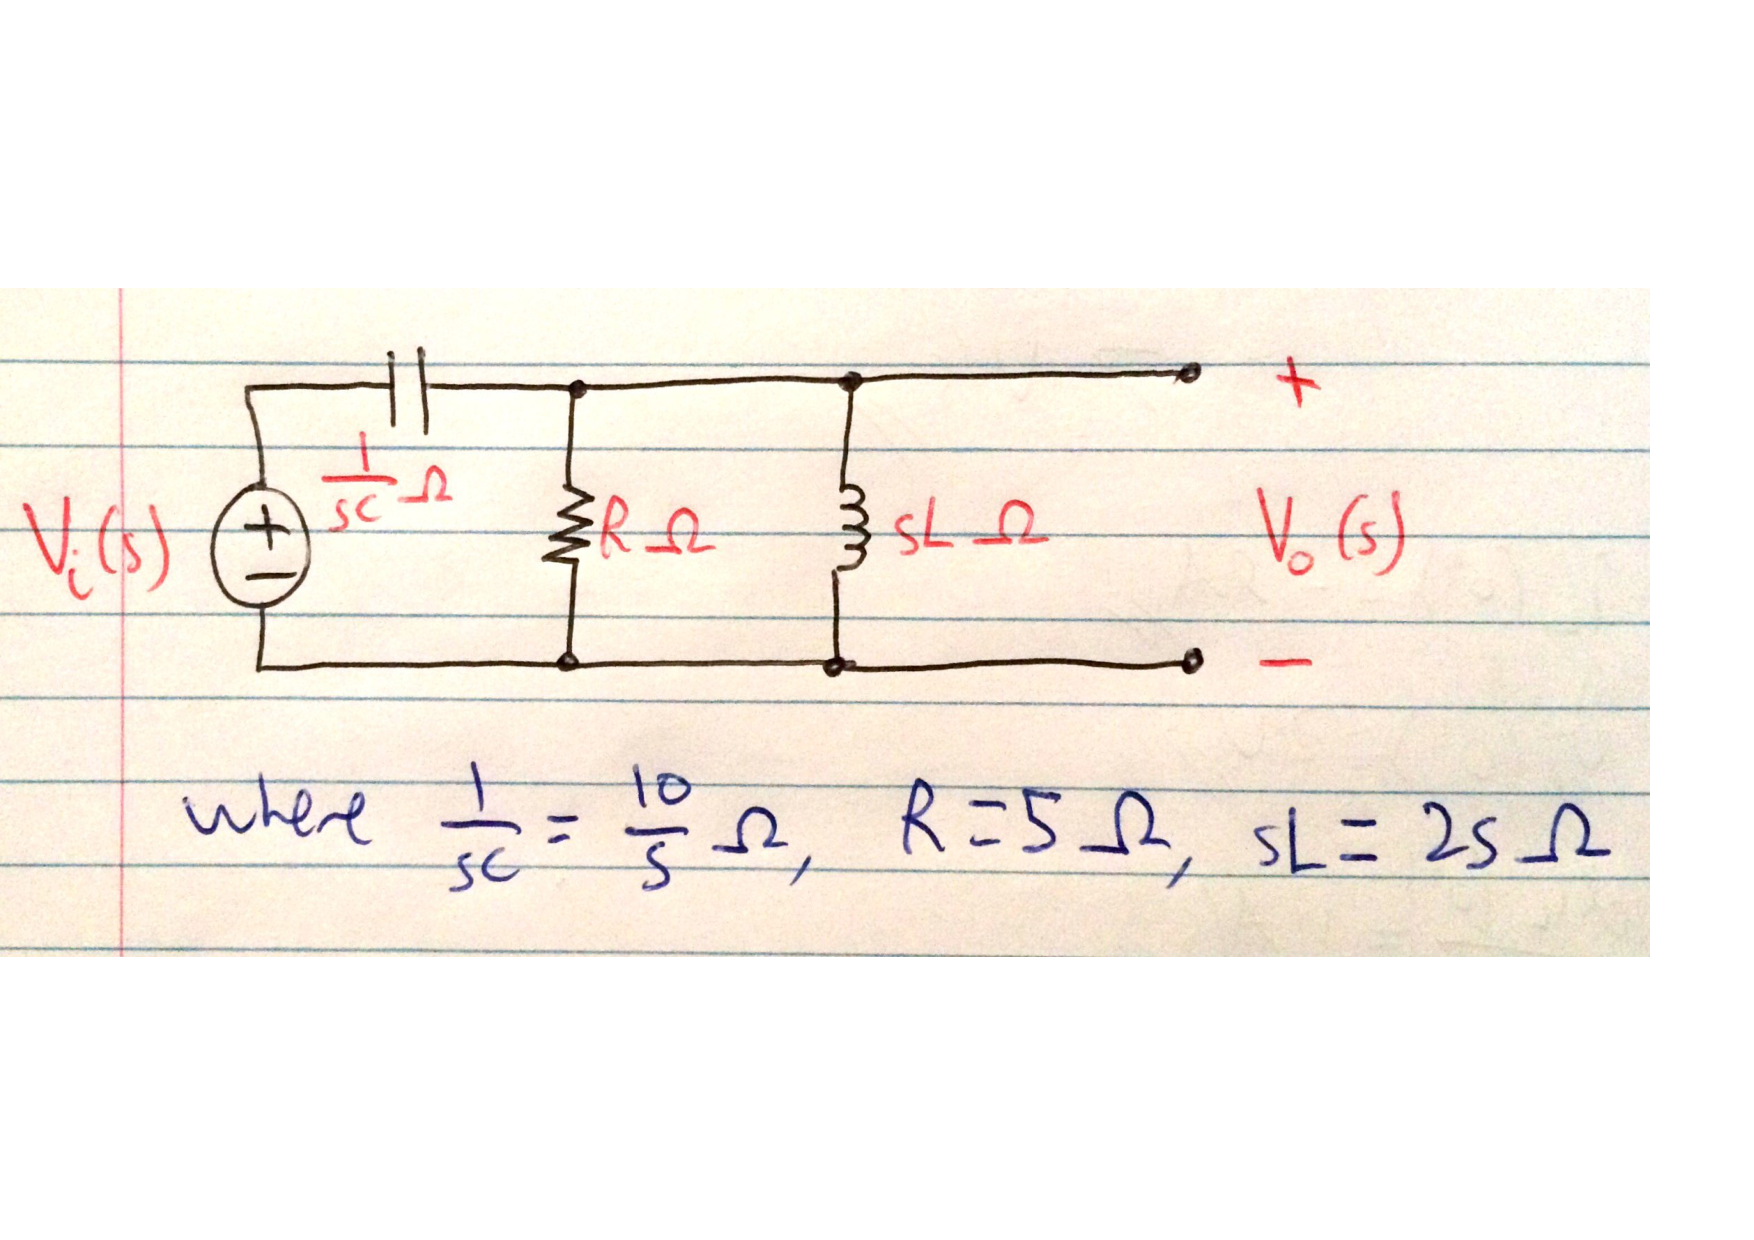
\includegraphics[scale=0.55]{q3a.pdf}
		\end{figure}
		Find $V_o(s)$ by recognising circuit is a voltage divider:
		\begin{align*}
			V_o(s) &= V_i(s) \times \frac{\frac{5\times2s}{5+2s}}{\frac{5\times2s}{5+2s} + \frac{10}{s}} \\ 
			\\
			\therefore H(s) &= \frac{10s}{10s+ \frac{50}{s} + 20} \\
			&= \frac{10s^2}{10s^2+20s+50} \\
			\\
			\therefore H(s) &= \frac{s^2}{s^2+2s+5}
		\end{align*}
		\\
	}

	\item{
	%Part b
		We note that the steady state response to the sinusoidal input will be given by the following equation:
		\begin{equation*}
			v_{oSS}(t) = 10 \times |H(j20)| \cos(20t + \theta(20))
		\end{equation*}
		\\
		Where $H(j\omega) = |H(j\omega)|e^{j\theta(\omega)}$
		\\ \\
		Therefore, find $|H(j20)|$ and $\theta(20)$:
		\begin{align*}
			H(j20) &= \frac{-400}{-395+j40} \\
			\\
			\therefore |H(j20)| &= \frac{400}{\sqrt{(-395)^2+40^2}} \\
			&= 1.008
		\end{align*}
		\begin{align*}
			\mathrm{And} \ \theta(20) &= \arctan \left(\frac{0}{-400} \right) - \arctan \left(\frac{40}{-395} \right) \\
			&= 180\degree - 174.22\degree \\
			&= 5.78\degree
		\end{align*}
		Finally sub these values into the equation for $v_{oSS}$:
		\begin{equation*}
			v_{oSS}(t) = 10.075 \cos(20t+5.78\degree) \ \mathrm{V}
		\end{equation*}
		\\
	}

\end{enumerate}
